% This is samplepaper.tex, a sample chapter demonstrating the
% LLNCS macro package for Springer Computer Science proceedings;
% Version 2.20 of 2017/10/04
%
\documentclass[runningheads]{llncs}
%
\usepackage{graphicx}
%\usepackage{geometry}
%\geometry{
%  a4paper,         % or letterpaper
%  textwidth=14cm,  % llncs has 12.2cm
%  textheight=22cm, % llncs has 19.3cm
%  heightrounded,   % integer number of lines
%  hratio=1:1,      % horizontally centered
%  vratio=2:3,      % not vertically centered
%}
% Used for displaying a sample figure. If possible, figure files should
% be included in EPS format.
%
% If you use the hyperref package, please uncomment the following line
% to display URLs in blue roman font according to Springer's eBook style:
% \renewcommand\UrlFont{\color{blue}\rmfamily}
\usepackage{amsmath}
\usepackage{algorithm}
\usepackage[noend]{algpseudocode}
\usepackage{tabu}
\usepackage{multirow, array}
% \setlength{\arrayrulewidth}{1pt}
%\setlength{\tabcolsep}{18pt}
%\renewcommand{\arraystretch}{1.5}

%\usepackage{rotating}
%\usepackage{array,makecell,multirow}
%\renewcommand\theadfont{\normalsize}% <-- added


% added by GN begin -->
	\usepackage{url}
	\usepackage{color}
	\def \GN#1{\textcolor{blue}{~#1}}	
% added by GN end 


\usepackage{array}
\newcolumntype{L}[1]{>{\raggedright\let\newline\\\arraybackslash\hspace{2pt}}m{#1}}
\newcolumntype{C}[1]{>{\centering\let\newline\\\arraybackslash\hspace{2pt}}m{#1}}
\newcolumntype{R}[1]{>{\raggedleft\let\newline\\\arraybackslash\hspace{2pt}}m{#1}}

\algnewcommand\algorithmicforeach{\textbf{for each}}
\algdef{S}[FOR]{ForEach}[1]{\algorithmicforeach\ #1\ \algorithmicdo}
\newcommand{\Break}{\State \textbf{break} }


\begin{document}
%
\title{Building Resource Auto-Scaler with Functional-Link Neural Network and Adaptive Bacterial Foraging Optimization}
%\title{A Novel Approach for Cloud Auto-scalers using FLNN and BFO-based Forecast and SLA-based Decision Making}
%\title{Designing Cloud Auto-scaling System with Functional-Link and  Neural Network for Multivariate Resources Metrics}
%
\titlerunning{Building Resource Auto-Scaler with Functional-Link and ABFOLS }
% If the paper title is too long for the running head, you can set an abbreviated paper title here



\author{Thieu Nguyen\inst{1}\orcidID{0000-0001-9994-8747}	\and
Binh Minh Nguyen\inst{1}\thanks{Corresponding author.}\orcidID{0000-0003-1328-3647} \and 
Giang Nguyen\inst{2}\orcidID{0000-0002-6769-0195}}
%
\authorrunning{T. Nguyen, B.M. Nguyen and G. Nguyen}
% First names are abbreviated in the running head.
% If there are more than two authors, 'et al.' is used.



\institute{School of Information and Communication Technology\\Hanoi University of Science and Technology, Hanoi, Vietnam\\
\email{nguyenthieu2102@gmail.com, minhnb@soict.hust.edu.vn}\\
\and
Institute of Informatics, Slovak Academy of Sciences, Bratislava, Slovakia\\
\email{giang.ui@savba.sk}}
%
\maketitle              % typeset the header of the contribution
%



\begin{abstract}

In this paper, we present a novel intelligent proactive auto-scaling solution for cloud resource provisioning systems. The solution composes of an improvement variant of functional-link neural network and adaptive bacterial foraging optimization with life-cycle and social learning
%for proactive resource utilization forecasting (FLABL). 
for proactive resource utilization forecasting as a part of our auto-scaler module. We also propose several mechanisms for processing simultaneously different resource metrics for the system. This enables our auto-scaler to explore hidden relationships between various metrics and thus help make more realistic for scaling decisions. In our system, a decision module is developed based on the cloud Service-Level Agreement (SLA) violation evaluation. We use Google trace dataset to evaluate the proposed solution well as the decision module introduced in this work. The gained experiment results demonstrate that our system is feasible to work in real situations with good performance.

\keywords{Proactive auto-scaling \and Functional-link neural network \and Adaptive bacterial foraging optimization \and Multivariate time series data \and Cloud computing \and Google trace dataset.}
\end{abstract}




%%%%%
\section{Introduction}
\label{intro}

Cloud technologies bring many benefits for both vendors and users. From the view of providers, they can maximize physical server utilization via time-sharing of using resources among multiple customers. Meanwhile, from the view of users, they do not need to care about infrastructure deployment costs, and only pay for what they used conforming to the pay-as-you-go model. Consequently, cloud hosting services are becoming more and more popular today.

One of the main outstanding features of cloud computing is the capability of elasticizing resources provided for applications. This mechanism thus supports to increase the availability as well as Quality of Service (QoS) for those applications~\cite{ref_hluchy}. Usually, the resource elasticity function is offered to users through an auto-scaling service that operates based on two techniques covering threshold and prediction. While the first already has been used in clouds, the second technique is still an attractive research problem today because there are barriers while applying the prediction-based auto-scaling system to clouds in practice. Firstly, accuracy of the prediction models must reach a certain level while having the ability of processing multiple resource metrics at the same time to meet practical demands. Secondly, the prediction models must be simple to deploy and operate but keep the effectiveness in forecast. Thirdly, the prediction-based auto-scaling system also must have a scaling decision mechanism which ensures QoS defined in Service-Level Agreement (SLA) signed between cloud customers and vendors. 


In this paper, we focus on developing a cloud prediction-based auto-scaler, which can simultaneously resolve the barriers presented above. In this way, our auto-scaler use a simple prediction model while still achieving the same level of accuracy and stability as compared with other complex methods. For the prediction module of the auto-scaler, we propose a novel variant of functional-linking neural network (FLNN) using adaptive bacterial foraging optimization with life-cycle and social learning (in short from here ABFOLS or Adaptive BFOLS) to train forecast model. Our prediction module also can simultaneously process multiple resources based on several data preprocessing mechanisms. To build scaling decision module for the auto-scaler, we exploit SLA-awareness to make decisions as well as evaluate these scaling actions. Our designed system is experimented and assessed with a real cluster trace dataset published by Google in 2011~\cite{clusterdata:Reiss2011}, and~\cite{ref_google_trace}. The gained outcomes show that our auto-scaler archives good performance and can be applied to practice.

The structure of this paper is as follows. In Section~\ref{related_work}, we classify and analyze existing studies to highlight our work contributions. Section~\ref{fl_bfonn} presents our cloud auto-scaler proposal (in short from here FLABL) with the intelligent core built based on the combination of FLNN and ABFOLS. The preprocessing raw data mechanisms, which helps the prediction module to exploit multiple data metrics is also described here. In the section~\ref{experiments}, we present tests and evaluations for the proposed auto-scaler to prove its effectiveness. The last section~\ref{conclusion} concludes and defines our future work directions.

\section{Related Work}
\label{related_work}
 
As mentioned in the previous Section, there are two cloud resources scaling mechanism types, namely reactive (i.e. systems will response to unpredictable resource consumption changes using usage thresholds) and proactive~\cite{ref_lorido} (i.e. systems attempt to predict resource requirements to make scaling decisions in advance). According to that classification, we focus on analyzing related works in the proactive technique category. 


\textbf{Resource consumption prediction}. 
In~\cite{ref_hipel}, several predictive time series models were proposed and demonstrated for cloud workload forecast problem such as ARMA (autoregressive-moving average), non-stationary, long memory, three families of seasonal, multiple input-output, intervention and multivariate ARMA models. As in~\cite{ref_vazquez}, the authors used two datasets collected from the Intel Netbatch logs and Google cluster data center to compare and evaluate prediction models together, including first-order autoregressive, simple exponential smoothing, double exponential smoothing, ETS, Automated ARIMA, neural network (NN) autoregression. Although these studies investigate methods for resource usage prediction, there is still lack of investigation of applying of FLNN variance in combination with evolutionary optimization in that domain like in~\cite{ref_thieu}.


\textbf{Functional-link neural network (FLNN).} 
Structurally, FLNN has only single neuron, which was proposed by Pao in~\cite{ref_pao} for pattern-recognition task. The network is quite simple but brings a good effective performance in the aspects of accuracy and training speed. Consequently, this learning model has been applied to many domains covering stock market prediction~\cite{ref_majhi}, and money exchange rate forecast~\cite{ref_rout}. In~\cite{ref_khan}, the authors used FLNN for four datasets of wine sales.
%namely average monthly temperature in New Delhi and India, monthly turnover in public services in Spain, and monthly Australian wine sales. 
The gained results prove that FLNN is more efficient in comparison with random walk model and feed-forward neural network (FFNN). The authors of~\cite{ref_sahoo} used FLNN with Chebyshev and Legendre polynomials to predict impact on tall building structure under seismic loads. The experiments presented in that work shown FLNN yields better outcomes as compared with multi-layer neural network (MLNN) also in terms of accuracy and computation time. However, the main disadvantage of FLNN is the use of back-propagation (BP) mechanism with gradients descent to train the learning model (\cite{ref_majhi},~\cite{ref_rout},~\cite{ref_khan}, and~\cite{ref_sahoo}) . 
 

\textbf{Adaptive Bacterial Foraging Optimization (ABFOLS).}
Recently, a new evolutionary computing technique called Bacterial Foraging Optimization (BFO) has been proposed in the work~\cite{ref_passino}. It is inspired based on principle of bacterial movement (i.e. tumbling, swimming or repositioning) to food-seeking. 
%(especially E. coli in the human intestine). 
Their behavior is achieved through a series of three processes on a population of simulated cells: "Chemotaxis", "Reproduction", and "Elimination-dispersal"~\cite{ref_passino}. BFO has been applied to several industry applications like PID controller tuning~\cite{ref_kim}, power system~\cite{ref_ali}, stock market~\cite{ref_ritanjali_majhi}. 
Unfortunately, BFO has certain shortages e.g., the appropriate time and method for dispersal and reproduction must be carefully selected, otherwise the stability of population may be destroyed~\cite{ref_yan}. 
%The algorithm is likely random search because the tumble angles of bacterium are generated randomly and their swarm also lacks interaction among others.
Therefore, the authors of~\cite{ref_yan} proposed an improvement for BFO including life-cycle of bacteria, social learning and adaptive search step length (ABFOLS), 
%involve which is called Adaptive Bacterial Foraging Optimization Algorithm with Lifecycle and Social Learning (Adaptive BFOLS or ABFOLS). 
which offer significant improvements over the original version in complexity and competitive performances as compared with other algorithms (e.g. GA) on higher-dimensional problems. 
%In terms of applying ABFOLS to real world problems, 
At present, there are no works that deal in optimizing FLNN with ABFOLS algorithm, especially in cloud auto-scaling issue.



\textbf{Cloud resources provision under SLA conditions.} In~\cite{ref_reig}, the authors presented a job scheduling system using machine learning to predict workloads and allocate resources complying with SLA. The authors of~\cite{ref_souza} used SLA to estimate the amount of resources required for making scaling actions. They argued that their algorithm is able to reduce the number of SLA violations up to 95$\%$ and decrease resource requirements up to 33$\%$. In~\cite{ref_dang}, the authors proposed a proactive cloud scaling system that enables to estimate SLA violations based on multiple metric parameters. Although the works~\cite{ref_reig}, and~\cite{ref_souza} already introduced SLA evaluation models, they operate based on single workload metric such as CPU usage, response time, or job execution deadline. Meanwhile, the work~\cite{ref_dang} allows processing multiple metrics, SLA violation still is evaluated based on resource usages (e.g. CPU, and memory usage). Conversely, in this study, we assess SLA to ensure QoS using the number of provided virtual machines (VMs). This is scaling unit, which cloud customers often care when making resources increase or decrease decisions. 

In comparison with the existing works analyzed above, the differences and contributions of our work are as follows. 
\begin{enumerate}
	\item Proposing an improvement (called FLABL) for FLNN, in which the network is trained by ABFOLS instead of back-propagation mechanism.
%	\item Proposing an improvement for FLNN (called FL-BFONN), in which the network is trained by BFO instead of back-propagation mechanism.
	\item Proposing an auto-scaler that uses  FLABL, %FL-BFONN
	which can process multivariate metric data and predict resource consumptions. 
	\item Proposing an SLA violation evaluation module that operates based on VM number rather than resource metrics in order to make scaling decisions for the proposed auto-scaler.
\end{enumerate}





%%%%%
\section{Resource auto-scaler using functional-link adaptive bacterial foraging optimization neural network}
%\section{Functional-link bacterial foraging optimization neural network}
\label{fl_bfonn}

%\subsection{Designing cloud auto-scaler}
\label{designing_system}

%The designs for our cloud auto-scaling system are shown by Fig.~\ref{FLBFONN_system} involving 4 phases: Cloud System, Extraction, Learning and Scaling. Scaling phase has two modules involving Forecasting and Decision.
The designs for our resource auto-scaling module are built based on underlying Cloud System. The module consists of 3 main phases, including Extraction, Learning and Scaling. The Scaling has two components namely Forecasting and Decision.



Raw resource monitoring data is collected from VMs in Cloud system. There are a lot of available monitoring services (e.g. CloudWatch, IBM cloud monitoring, and Rackspace Monitoring, Nagios, Prometheus and Zabbix and so forth) that can be used or deployed on cloud infrastructures for monitor problem. Based on the monitoring services, we gather diverse VM metrics such as CPU, memory utilization, disk IO, network IO, etc.). The detail descriptions of Extraction, Learning and Scaling phases are described in the following subsections. 

\subsection{Extraction phase}
\label{extraction_phrase}

There are seven mechanisms deployed in Extraction phase to pre-process raw data and prepare normalized data for Scaling phase in our system. As shown in Fig.~\ref{FLABLextraction}, those mechanisms cover: 

\begin{figure}
	\begin{center}
		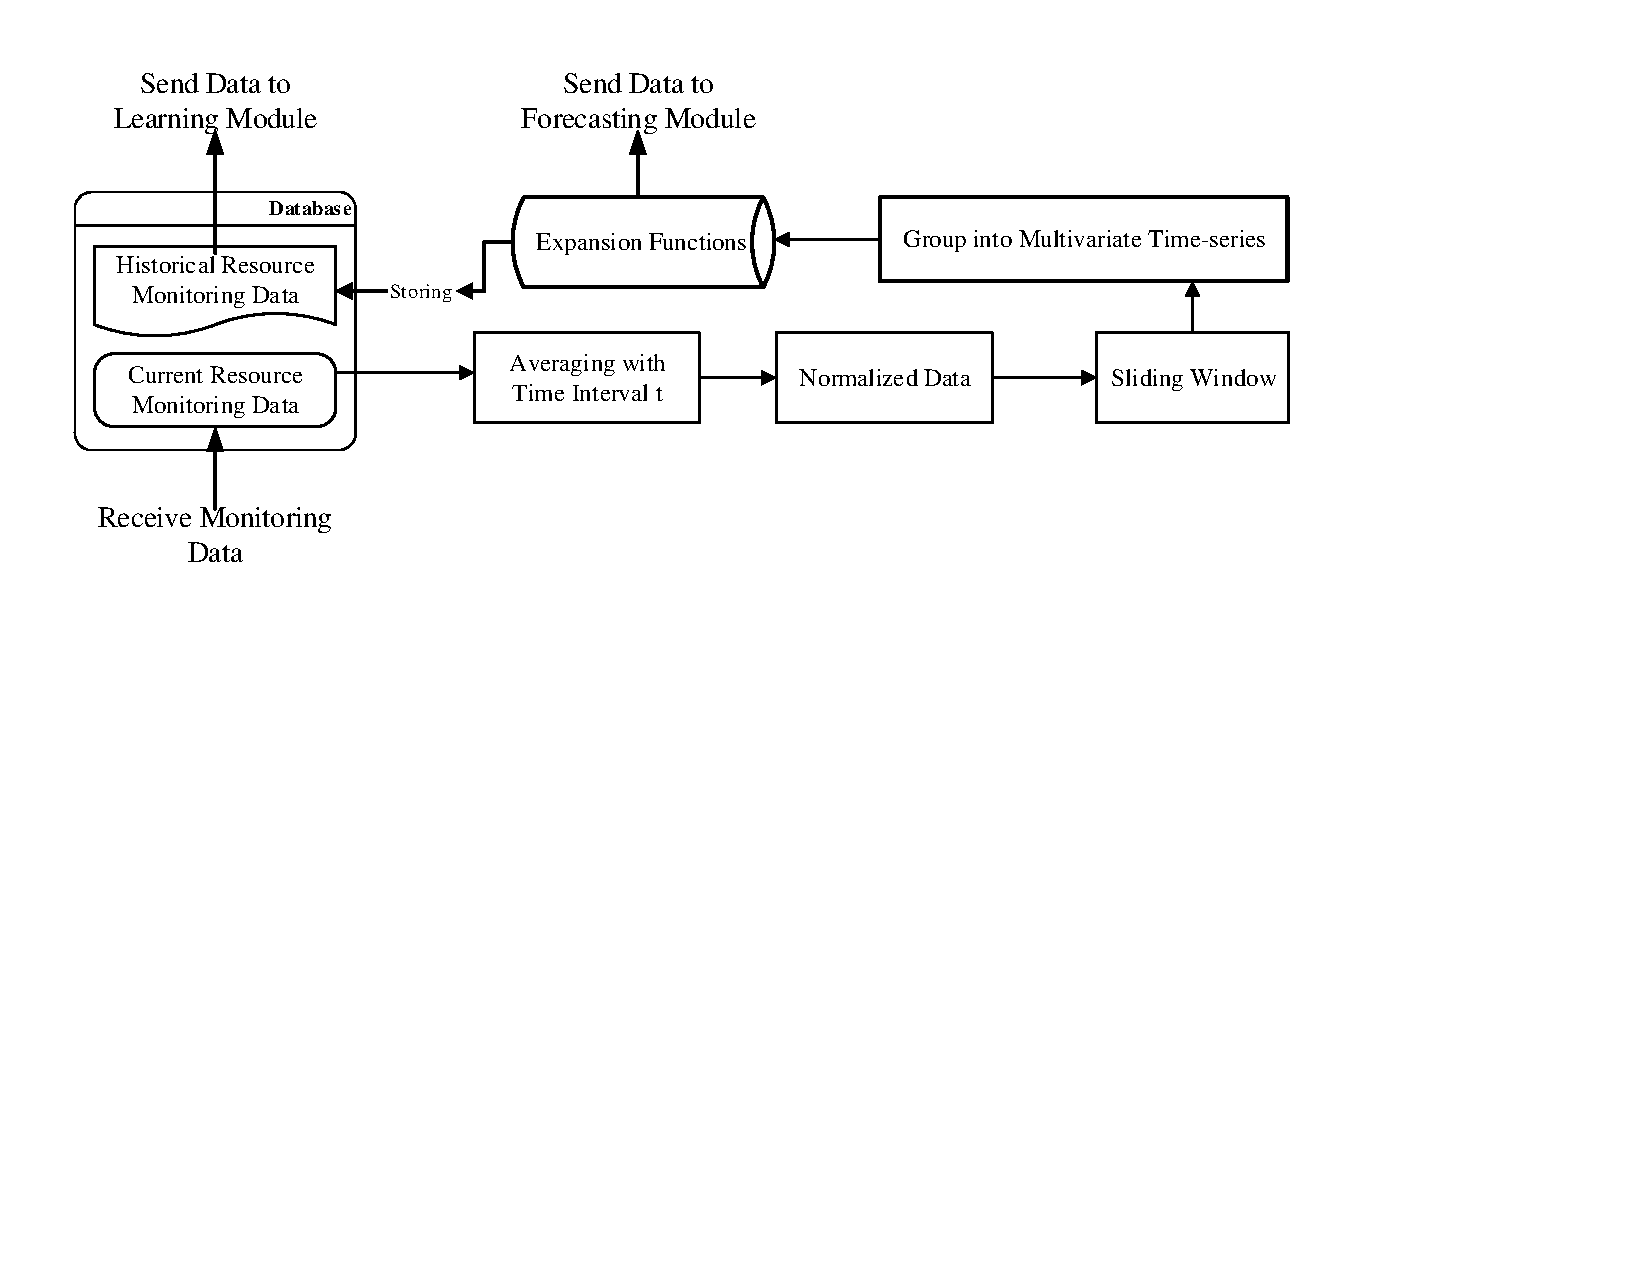
\includegraphics[width=0.9\textwidth =0cm 0cm 0cm 0cm, clip]{images/pdf/Extraction_Module.pdf}
		\caption{FLABL data extraction process}
		\label{FLABLextraction}
	\end{center}
\end{figure}


\begin{enumerate}
	\item Using collected raw monitoring data from the underlying Cloud System. 
	\item Transforming current raw data in the predefined period for model training into corresponding time series $r_i(t) (i = 1, 2,..., M)$ with time interval $\rho$. 
	\item Averaging values of given metrics in the given interval of $\rho$ for each point in time series $r_i(t)$.
%as follows: $r_i(n) = \frac{ \sum_{i=(n-1)\rho < t < n\rho}^nD_i(t) }{ n_{\rho} }$, where $D_i(t)$ is the value of type-i metric at time $t$ that is monitored from cloud system, $n\rho$ is the number of observation $D_i(t)$ in interval $\rho$. 
	\item Normalizing the time series data in the range of [0, 1]. 
	\item Transforming the normalized time series data to supervised data using sliding technique with window width $k$, which is the number of used values before the time $t$ to predict a value at the time $t$. 
%Dealing with the multiple metrics processing, all metric types are grouped into single multivariate data in the next mechanism. 
	\item  
%because there is no a hidden layer in the neural network structure, 
The supervised data undergoes through an expansion function (e.g. Chebyshev or Power series) to enable the ability of catching nonlinear relationship between inputs and outputs. 
	\item Finally, the output data is put into a database in form of historical resources data, which is used to build prediction model in Learning phase. The data also is provided for Forecasting module in Scaling phase to predict the resource consumption.
\end{enumerate}

\subsection{Learning phase}
\label{learning_phase}
Generated data from Extraction phase is divided into three different sets, namely training, validating, and testing. While the first two sets are employed to learn and select parameters, the third set is used for validating trained prediction model. 
%As presented before, 
%The proposed model is taken shape from FLNN (in Extraction phase) and is optimized by ABFOLS as described in Algorithm~\ref{algo_BFO}.  
A novel method is proposed in our Learning phase based on FLNN and trained by ABFOLS algorithm to speed up the convergence and increase the prediction accuracy. Due to combinations, our learning method is called by Functional-Link Adaptive Bacterial Foraging Lifecycle Neural Network (called by FLABL).

The final trained model of Learning is used in Forecasting module that belongs to Scaling phase. Meanwhile, the real-time monitoring data collected from cloud VM after preprocessing will be use as Real-time monitoring resource usage before putting into our Final Model of Forecasting module. The gained predictive results then will be denormalized to be able to use in the next module.


\begin{figure}
	\begin{center}
		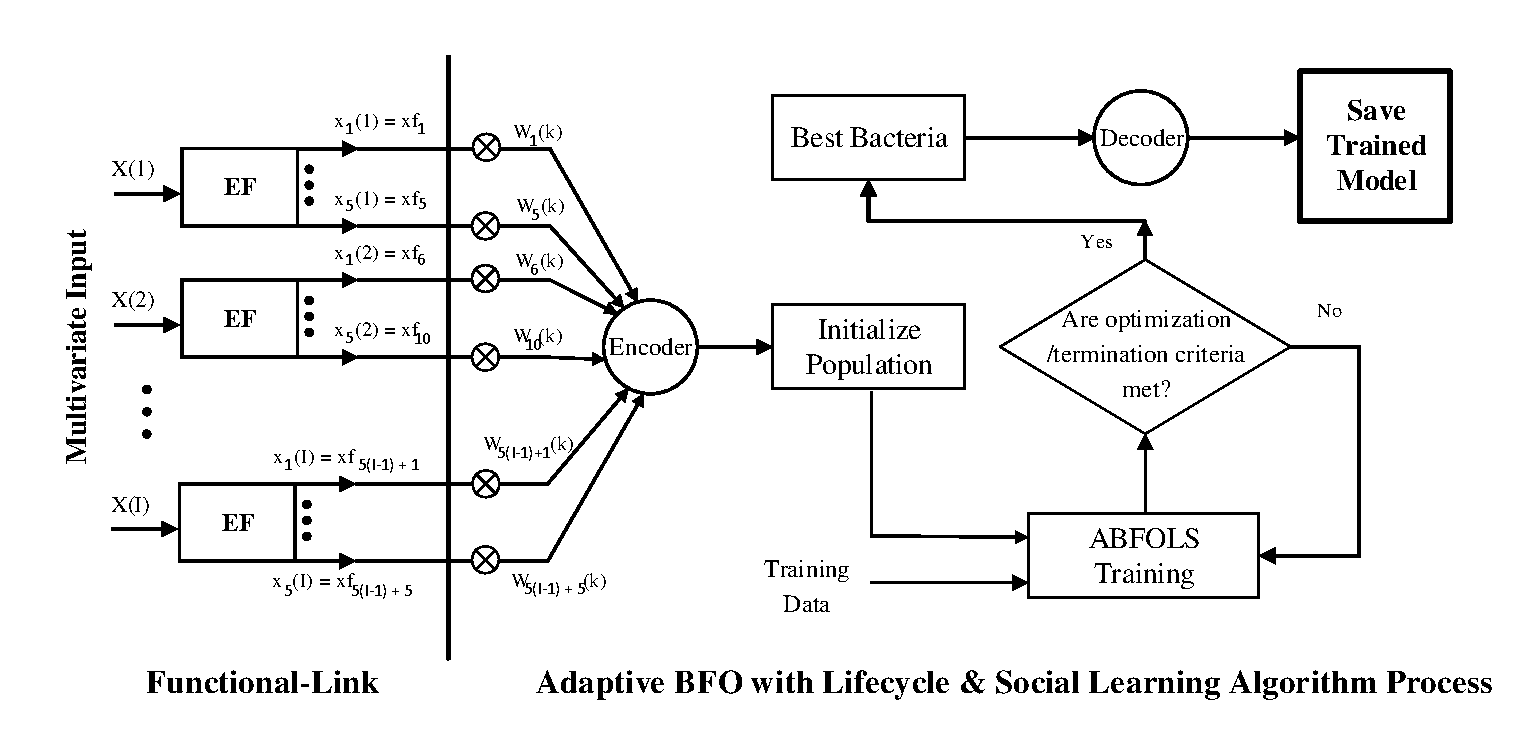
\includegraphics[width=1.0\textwidth =0cm 0cm 0cm 0cm, clip]{images/pdf/FLBFONN_training.pdf}
		\caption{ FLABL Learning phase with FLNN and ABFOLS }
		\label{FLBFONN_process}
	\end{center}
\end{figure}


\begin{algorithm}
	\caption{FLABL Learning phase }\label{algo_BFO}
	\hspace*{\algorithmicindent} \textbf{Input:} 
	\textbf{ $S$, $N_s$, $P_{ed}$, $C_s, C_e$, $N_{split}, N_{adapt}$ }
	
	\hspace*{\algorithmicindent} \textbf{Output:} The trained model
	
	\begin{algorithmic}[1]
		\State Normalizing all current resource time series of $M$ type of resource consumption: 
			\Statex $r_1(t),r_2(t),...,r_i(t),...,r_M(t)$
		
		\State Initializing sliding window with $p$ consecutive points as the inputs 
			\Statex $(X_1(t), X_1(t-1), ..., X_1(t-p+1)),..., (X_M(t), X_M(t-1), ..., X_M(t-p+1))$  
			\Statex and the next observation 
			\Statex $X_1(t+k), ..., X_M(t+k)$ as the outputs $(t = 1,2,...,n)$
		
		\State Grouping all column inputs data of $M$ type resource into multivariate data
			\Statex $X(t) = [ X_1(t), X_1(t-1), ..., X_1(t-p+1), ..., X_M(t), X_M(t-1), ..., X_M(t-p+1) ]$
		
		\State Applying expansion functions to multivariate data: 
			\begin{equation}
				\begin{split}
			x(t) = [ x_1^1(t), x_1^2(t), ..., x_1^5(t), x_1^1(t-1), x_1^2(t-1), ..., x_1^5(t-p+1), ..., \\
				  x_M^1(t), x_M^2(t), ..., x_M^5(t), x_M^1(t-1), x_M^2(t-1), ..., x_M^5(t-1), ..., \\
				  x_M^1(t-p+1), x_M^2(t-p+1),.., x_M^5(t-p+1) ]
				\end{split}
			\end{equation}
		
		\State Training the constructed FLNN (from step 1 to 4) by ABFOLS (from step 6 to 31)
		
		\State Initialize population $Pop$ = $ \left\{ Cell_1,. . . , Cell_{s} \right\}$ with $S$ cells ($bacterium$),
			\Statex where $Cell_i = (c_{i1}, …, c_{id})$, $c_{ij} \in [-1, 1]$ with $d$-dimensions, $d = length(x(t) + 1)$
			\Statex Initialize $Nutrient(i) \gets 0$ for all $Cell_i$
			
		\While {(termination conditions are not met)}
			\State $S \gets size(Pop)$; i $\gets$ 0  						% size of the last population
			\While {($ i < S $)}
				\State $ i \gets i+1$; $ fitLast \gets fitCurrent(i) $ 
				\State Generate a tumble angle for $Cell_i$ by Eq.~\ref{eq_social}
				\State Update the position of $Cell_i$ by Eq.~\ref{eq_position}
				%\State Recalculate the fitness and the nutrient of bacterium i 
				\State Recalculate $fitCurrent(i)$ and $Nutrient(i)$ 
				\State Update personal best ($Cell_{pBest}$) of ith cell and global best ($Cell_{gBest}$)
				
				\For{\texttt{ m = 1 to $N_s$ }}
					\If{ $fitCurrent(i) < fitLast$ }
						\State $fitLast \gets fitCurrent(i)$
    						\State Run one step using Eq.~\ref{eq_position}		% Run one more step
    						%\State Recalculate the fitness and the nutrient of bacterium i
    						\State Recalculate $fitCurrent(i)$ and $Nutrient(i)$
    						\State Update $Cell_{pBest}$ and $Cell_{gBest}$
  					\Else
  						\Break
  					\EndIf
				\EndFor
			\EndWhile
			
			\If{ $Nutrient(i) > threshold_{split}$ (Eq.~\ref{eq_split} is True) }
    				\State Split $Cell_i$ into two $cell$ 
    				\Break
  			\EndIf
  			
  			\If{ $Nutrient(i) < threshold_{dead}$ (Eq.~\ref{eq_dead} is True) }
    				\State Remove $Cell_i$ from $Pop$
    				\Break
  			\EndIf
  			
  			\If{ $Nutrient(i) < 0$ and $random(0, 1) < P_{e}$ }
    				\State Move $Cell_i$ to a random position
  			\EndIf
  		\EndWhile
		\State Passing the \textbf{trained model} ($Cell_{gBest}$) to Forecasting module.
		\State Repeating step 1 to step 30 in every time period $T$
	\end{algorithmic}
\end{algorithm}

The details of our proposal FLABL are as follows: Used parameters in Algorithm~\ref{algo_BFO} are explained in Table~\ref{table:bfo_paras}. While$Nutrient(i)$ is the nutrient of ith bacterium, $fitCurrent(i)$ is the current fitness value of ith bacterium, $fitLast$ is the fitness value of the last position of ith bacterium, $Cell_{pBest}$ is the past position of ith, bacterium which gained the best fitness so far. $threshold_{split}$ and $threshold_{dead}$ is coresponding to right side of Eq.~\ref{eq_split} and Eq.~\ref{eq_dead}.

We use Mean Absolute Error (MAE) for bacterial fitness function according to the Eq.~\ref{eq_mae}. In chemotactic steps, a bacterium will update its position based on the direction which created by combination of information of its personal best position and the population’s global best position in Eq.~\ref{eq_position} and Eq.~\ref{eq_social}. The gain of nutrients process is updated when bacteria move, so if the new position is better than the last one (the fitness higher), it is regarded that the bacterium will gain nutrient from the environment and the nutrient is added by one. Otherwise, it loses nutrient in the searching process and its nutrient is reduced by one Eq.~\ref{eq_nutrition}.

In an intelligence optimization algorithm, it is important to balance its exploration ability and exploitation ability. In the early stage, we should enhance the exploration ability to search all the areas. In the later stage of the algorithm, we should enhance the exploitation ability to search the good areas intensively. So in BFO, the step size which bacterium used to move play an important role. We use the decreasing step length based on bacterium's fitness (Eq.~\ref{eq_step_size_general}). In the early stage of BFOLS algorithm, larger step length provides the exploration ability. And at the later stage, small step length is used to make the algorithm turn to exploitation. Besides, we also deploy an adaptive search strategy, which change the step length of each bacteria based on their own nutrient, which calculated using (Eq.~\ref{eq_step_size_i}). The higher nutrient value, the bacterium’s step length is shortened further. This is also in accordance with the food searching behaviors in natural. The higher nutrient value indicates that the bacterium is located in potential nutrient rich area with a larger probability. So, it is necessary to exploit the area carefully with smaller step length.




\small
%\scriptsize
\begin{equation} \label{eq_mae}
fit = MAE = \frac{\sum_{i=1}^N|forecast(i) - actual(i)|}{N}
\end{equation}

\begin{equation} \label{eq_position}
\theta^{t+1}_i = \displaystyle \theta^t_i + C(i) * \frac{\Delta_i}{ \sqrt{ \Delta_i * \Delta^T_i } } 
\end{equation}

\begin{equation} \label{eq_social}
\Delta_i = ( \theta_{gBest} - \theta_i ) + ( \theta_{i,pBest} - \theta_i ) 
\end{equation}

\begin{equation} \label{eq_nutrition}
Nutrient(i) = \begin{cases}  Nutrient(i) + 1, & \mbox{if } fitCurrent(i) > fitLast\\ Nutrient(i) - 1, & \mbox{if } fitCurrent(i) < fitLast \end{cases}
\end{equation}

\begin{equation} \label{eq_split}
Nutrient(i) > \displaystyle max\Big( N_{split}, N_{split} + \frac{S^i - S}{ N_{adapt} } \Big)
\end{equation}

\begin{equation} \label{eq_dead}
Nutrient(i) < \displaystyle min\Big( 0, 0 + \frac{S^i - S}{ N_{adapt} } \Big)
\end{equation}

\begin{equation} \label{eq_step_size_general}
C = \displaystyle C_s - \frac{ (C_s - C_e) * nowFit }{ totalFit } 
\end{equation}

\begin{equation} \label{eq_step_size_i}
C(i) = \begin{cases}  \displaystyle \frac{C}{Nutrition(i)} , & \mbox{if } Nutrient(i) > 0\\ C, & \mbox{if } Nutrient(i) \leq 0 \end{cases}
\end{equation}
\normalsize

\begin{table}[!h]
\begin{center}
\begin{tabular}{ |C{2cm}| C{10cm} | } 
\hline
\textbf{Name} & \textbf{Description} \\ \hline
$S$ & The number of cells (bacteria) in the population \\ \hline
$d$ & $d$-dimension / problem size \\ \hline
$N_s$ & Swimming length after which tumbling of bacteria will be undertaken in a chemotactic loop \\ \hline
$P_{ed}$ & Probability for eliminate bacteria \\ \hline
$C_s, C_e$ & The step size at the beginning and the end of chemotactic process\\ \hline
$N_{split}, N_{adapt}$ & Parameters used to control and adjust the split criterion and dead criterion. \\ \hline
\end{tabular}
\end{center}
\caption{FLABL parameters used for ABFOLS optimization}
\label{table:bfo_paras}
\end{table}




\subsection{Scaling phase}
\label{scaling_phase}

The Scaling phase contains of Forecasting and Scaling components. The functionalities and collaboration of these two components are based on SLA-violation auto-scaling strategy as described in Algorithm~\ref{algo_auto_scaling}.

\begin{figure}
	\begin{center}
		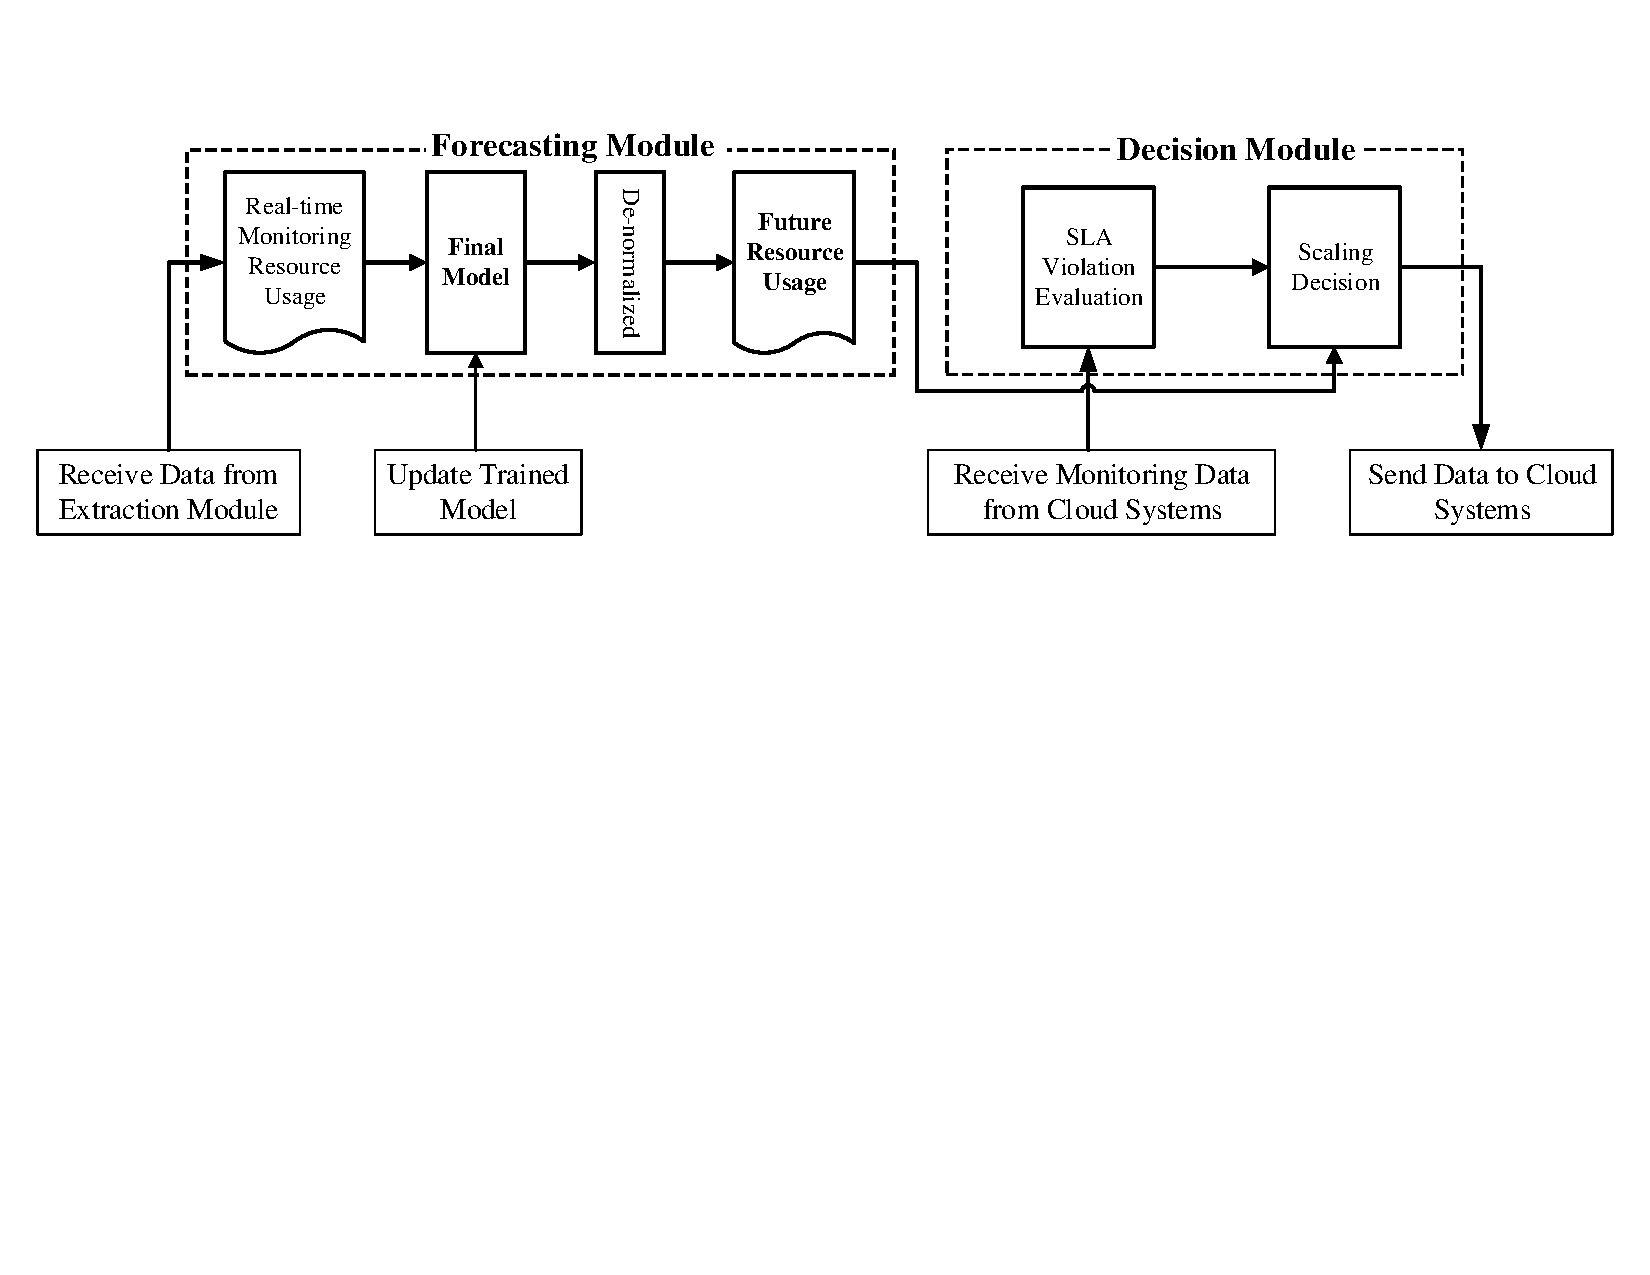
\includegraphics[width=1.0\textwidth =0cm 0cm 0cm 0cm, clip]{images/pdf/Forecasting_Module.pdf}
		\caption{FLABL Scaling phase}
		\label{FLABLscaling}
	\end{center}
\end{figure}


\begin{algorithm}[thb]
	\caption{Auto-scaling strategy based on SLA-violations}\label{algo_auto_scaling}
	\begin{algorithmic}[1]
		\State At each timepoint $t$, calculate 
			$F^{pred}_{1}(t+1), F^{pred}_{1}(t+1), .., F^{pred}_{1}(t+1)$ by FLABL 
			\Statex then de-normalize results back to get resources consumption at the next timepoint:
			$r^{pred}_{1}(t+1), r^{pred}_{2}(t+1), ..., r^{pred}_{i}(t+1)$
		\State Calculating the number of VMs predicted at time $(t+1)$ as 
%			equation (\ref{eq_vm_predictions})
			\begin{equation} \label{eq_vm_predictions}
				n^{pred}_{VM} (t+1)  = 
				max \Big\{ \frac{ r^{pred}_{1}(t+1) }{ C_1 }, \frac{ r^{pred}_{2}(t+1) }{ C_2 },.., \frac{ r^{pred}_{i}(t+1) }{ C_i } \Big\}
			\end{equation}	
		\State \textbf{for} $(z \gets t-L+1)$ to $t$ calculate the number of VMs violations  
%			based on equation (\ref{eq_vm_violations})
			\begin{equation}\label{eq_vm_violations}
				n^{violation}_{VM} (t) = max \big\{  0, n^{actual}_{VM} (t) - n^{alloc}_{VM} (t)  \Big\}
			\end{equation}
		\State Calculating the number of allocated VMs 
%			$n^{alloc}_{VM} (t+1)$ 
%			by equation (\ref{eq_vm_allocated})	
			\begin{equation}\label{eq_vm_allocated}
				n^{alloc}_{VM} (t+1) = s * n^{pred}_{VM} (t+1) + \frac{1}{L} \displaystyle\sum_{z=t-L+1}^t n^{violation}_{VM} (z)
			\end{equation}
		\If{ $ n^{alloc}_{VM} (t+1) > n^{alloc}_{VM} (t) $ }
			\State Making decision to instantiate $ n^{alloc}_{VM} (t+1) - n^{alloc}_{VM} (t) $ VMs
		\Else
			\State Making decision to destroy $ n^{alloc}_{VM} (t) - n^{alloc}_{VM} (t+1) $ VMs
		\EndIf
		\State Repeating from step 1 to 8 at the next point of time.
	\end{algorithmic}
\end{algorithm}


\subsubsection{Forecasting module}
\label{forecasting_module}
Forecasting phase uses real-time monitoring data (is preprocessed by Preprocessing phase) as inputs for the trained model to predict new values (i.e. resource consumption) in advance. Then, the obtained outputs are de-normalized into the real values. In every time period $T$, learning algorithm is updated with new monitoring data.


\subsubsection{Decision module}
\label{decision_module}
Decision module is responsible for calculating the number of provided VMs according to the predictive resource consumption. In addition, we develop SLA Violation Evaluation component that operates based on the number of VMs allocated at previous time and with the VM numbers predicted in the future to decide the how many VMs will be provisioned as in Equations~\ref{eq_vm_predictions}, \ref{eq_vm_violations}, and \ref{eq_vm_allocated}. 
Finally, predictive scaling information will be sent to Resource Scaling Trigger in Cloud System to create appropriate actions.
With resource usages predicted by Forecasting module, we assume that cloud system can provision unlimited amount of VMs like the systems presented in~\cite{ref_nguyen}, which has the same hardware configuration. We also do not consider VM scheduling policies in our scaling strategy in this work. 


In terms of QoS guarantee, the number of predicted VMs will be multiplied by $s$ ($s$ $\ge$ 1). The larger $s$, the more VMs allocated to applications and this reduces the SLA violations. In this direction, the total number of SLA violations in an earlier period with length $L$ is used to determine the increases (or decreases) of allocated VMs. 
%Our auto-scaling strategy is presented by Algorithm~\ref{algo_auto_scaling}.



%%%%%
\section{Experiments}
\label{experiments}
To evaluate our proposed auto-scaler, we carry out two experiments, including:

\begin{enumerate}
	\item Comparing prediction accuracy and the system run time between various neural network models with our FLABL, involving ANN, MLNN, traditional FLNN, FL-GANN and FL-BFONN using univariate and multivariate data. 
	\item Evaluating scaling performance of our proposed auto-scaler under SLA violation measurement.
\end{enumerate}
%	\item Evaluating influence of SLA-violations parameters on the auto-scaling strategy used in our system.



\subsection{Experimental setup}
\label{experimental_setup}

\textbf{Dataset.} In our experiment, we use dataset gathered by Google from one of their production data center clusters. The log records operations of approximate 12000 servers for one month~\cite{clusterdata:Reiss2011}, \cite{ref_google_trace}. This log thus contains a lot of jobs submitted to the cluster. Each job is a collection of multiple tasks that are run simultaneously on many machines. Resource utilization of tasks is measured by several metrics such as CPU, and memory usage, disk I/O, and so on with more than 1233 million data items. To evaluate our predictive model as well as the auto-scaling strategy, we chose a long-running job with ID 6176858948, which consists of 60171 divergent tasks during the 20-day period. 

\begin{figure}
	\centering
	\begin{minipage}[t]{6cm}
		\centering
		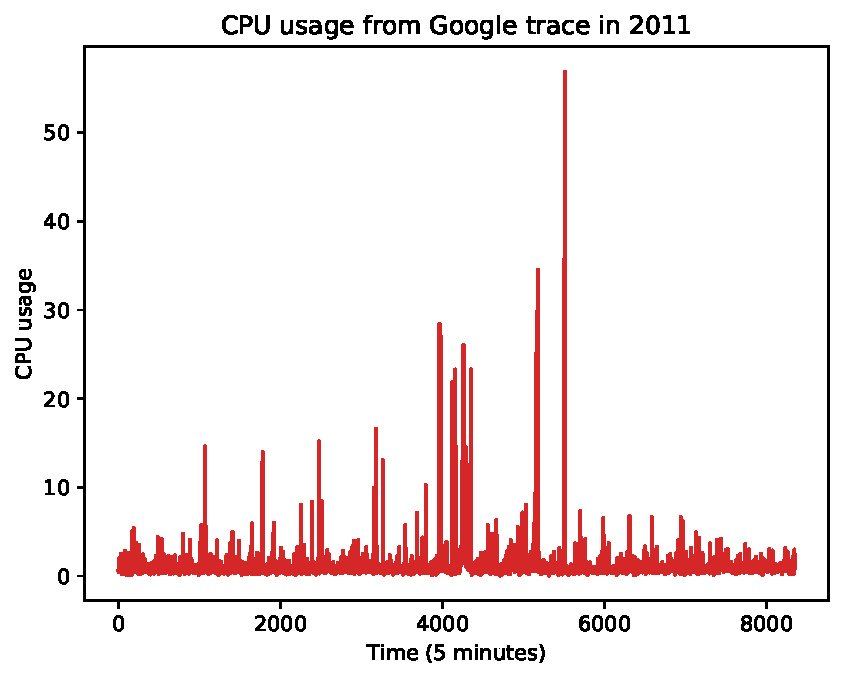
\includegraphics[width=1\textwidth =0cm 0cm 0cm 0cm]{images/pdf/google_cpu_5m.pdf}
	\end{minipage}
	\begin{minipage}[t]{6cm}
		\centering
		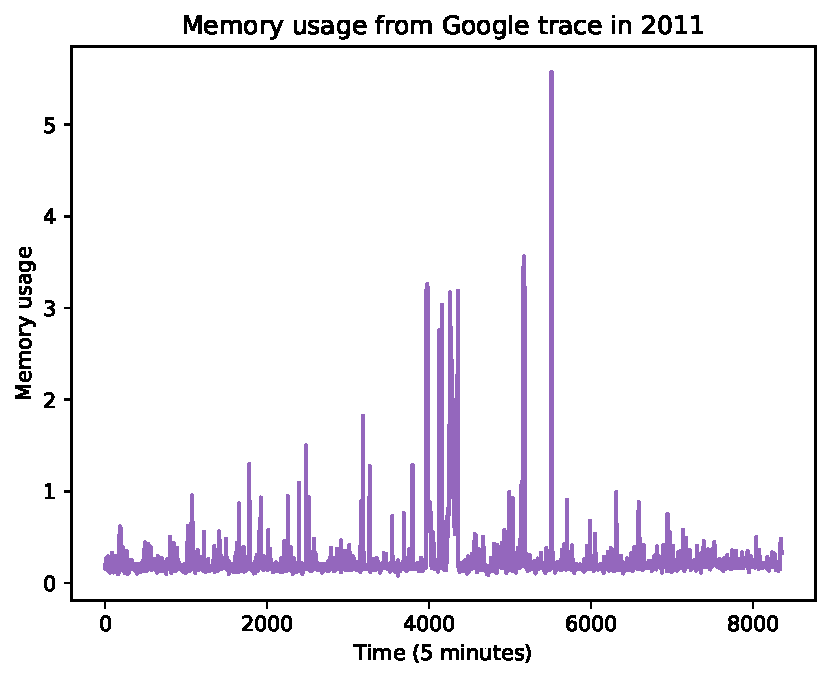
\includegraphics[width=1\textwidth =0cm 0cm 0cm 0cm]{images/pdf/google_ram_5m.pdf}
	\end{minipage}
	\caption{CPU(left) and memory(right) from Google trace dataset (Google normalized data) } 
	\label{fig_dataset}
\end{figure}

We assume that the cloud system has enough VMs to process the chosen long-running job. VM capacity is equal to the minimum configuration of a machine in Google cluster with $C_{CPU}$ = 0.245 and $C_{RAM}$ = 0.03 (normalized values). We also assume that time required to instantiate a new VM is five minutes. Therefore, the resource usages in the incoming five minutes are predicted to make scaling decisions in advance. In this way, average time $t$ is set by 5 minutes, forecast horizon $k$ = 1 in all experiments. While, the collected data from $1^{st}$ to $14^{th}$ day is used to train the networks, data from $15^{th}$ to $17^{th}$ day employed to validate network's parameters, and data from $18^{th}$ to $20^{th}$ day is used to test the prediction performance. We select both CPU and memory metric types (visualization in Fig.~\ref{fig_dataset}) in the Google dataset as multivariate data for our proposed system. Before we group CPU and memory data to be multivariate data, we make sure the data range in the same by normalized step in the Extraction phrase. The prediction accuracy is assessed by Root Mean Square Error $RMSE = \sqrt{  \frac{\sum_{i=1}^N( forecast(i) - actual(i) )^2}{N} }$.

\textbf{Test models.} Our tested ANN model is cofigured with three layers (one input, one hidden, and one output), MLNN model is configured with five layers (one input, three hidden and one output). Meanwhile, FLNN, FL-GANN, FL-BFONN and FLABL have only one input and output layer with structure $(x, 1)$. The polynomial is set as functional-link for all models. Here, $x$ is the sliding window value used in the Extraction phase in our system. Activation function used for our tested networks are Exponential Linear Unit (ELU)~\cite{ref_clevert}.

Based on previous research in~\cite{ref_thieu}, we use standard GA algorithm for FL-GANN model. The GA parameters are set as follows. The population size $p_s$ = 500, the maximum number of generations $g_{max}$ = 700, the probability of two individuals exchanging crossovers $p_c$ = 0.95 and the probability of individual mutation $p_m$ = 0.025. For BFO algorithm, the parameters are configured in the same way as works described in~\cite{ref_passino} which are set as follows: The length of the lifetime of the bacteria as measured by the number of chemotactic steps they take during their life $N_c = 50$, swimming length after which tumbling of bacteria will be undertaken in a chemotactic loop $N_s = 4$, maximum number of reproduction to be undertaken $N_{re} = 4$, the number of elimination-dispersal steps $N_{ed} = 8$, probability for eliminate bacteria $P_e = 0.25$, and $Step_{size} = 0.1$. Finally, for our ABFOLS algorithm, the parameter settings are similar to~\cite{ref_yan} work which are $N_s$ = 4, $P_e$ = 0.25 (same as BFO configurations), $N_{split}$ = 30, $N_{adapt}$ = 5, the step size at the beginning of process $C_s$ = 0.1($U_b$ - $L_b)$, the step size at the end of the process $C_e$ = 0.00001($U_b$ - $L_b$), where $U_b$ and $L_b$ are referred to the upper and lower bound of the variables. 




\textbf{SLA evaluation mechanisms.} We use SLAVTP (SLA Violation Time Percentage) proposed in~\cite{ref_dang} to evaluate our proposed VM calculation mechanism (formula~\ref{eq_vm_allocated} 
	$ SLAVTP = \frac{T_{under-provisioning}}{T_{execution}}$, where 
	$T_{under-provisioning}$ is the time when at least one allocation resource causes "under-provisioning" (i.e. lack of RAM or CPU core), and 
	$T_{execution}$ is total time of the application running in cloud system. 

To evaluate performance of our auto-scaling strategies, we use ADI (Auto-scaling Demand Index) measurement~\cite{ref_netto}, 
which considers the difference between actual and desired resource utilization. In other words, the total distance between $u_t$ and $[L, U]$. In which $u_t$ is the utilization level of the system, $L$ and $U$ correspond to the lower and upper limits of reasonable resource use, with $0 \le L \le U \le 1.0$. The ADI is denoted by the variable $\sigma = \sum_{t \in T}{\sigma_t}$ where, $\sigma_t = L - u_t$ if $u_t \le L$; $\sigma_t = 0$ if $L < u_t <U$; $\sigma_t = u_t -U$ if otherwise. For each time $t$, according to the ADI formula, the optimization strategy will yield a minimum of $\sigma$. 

\subsection{FLABL forecast accuracy and runtime}
\label{predicting_results}

In this test, we evaluate the efficiency of FLABL against FL-BFONN, FL-GANN, traditional FLNN, MLNN and ANN in forecasting resources consumption. For each model, we use both univariate (single input metric) and multivariate (multiple input metrics) data. We also change sliding windows size $k$ from 3 to 5 ($k$ = 3, 4, 5) in the experiment to test effectiveness fluctuation. Our achieved outcomes are given in Table~\ref{table:forecasting_results}.

\begin{table}[!h]
\begin{center}
% \begin{tabular}{| c | c| L{5cm} | C{3cm} | R{6cm} |}
\begin{tabular}{| c | c| C{1.2cm} | C{1.2cm} | C{1.2cm} | C{1.2cm} | C{1.2cm} | C{1.2cm} |}
 \hline
  \multirow{2}{*}{Input Type} & \multirow{2}{*}{Model} & \multicolumn{3}{c|}{CPU} & \multicolumn{3}{c|}{RAM} \\ \cline{3-8}
   & & k = 3 & k = 4 & k = 5 & k = 3 & k = 4 & k = 5  \\ [0.5ex] \hline
 \multirow{5}{*}{ Univariate } & ANN	& 0.4962  & 0.4952  & 0.5054  & 0.0344 	& 0.0352 	& 0.0354  \\  
 & MLNN	& 0.4903  & 0.4930  & 0.4966	& 0.0345 	& 0.0349 	& 0.0355  \\  
 & FLNN	& 0.5171  & 0.510  & 0.5253	& 0.038 	& 0.0356 	& 0.0373  \\  
 & FL-GANN	& 0.4892  & 0.4762  & 0.4877	& 0.0389 	& 0.0376 	& 0.0375  \\ 
 & FL-BFONN	& 0.4777  & 0.4872  & 0.4798	& 0.0342 	& 0.0431 	& 0.035  \\ 
 & FLABL	& \textbf{0.469}  & \textbf{0.4726}  & \textbf{0.4732}	 & \textbf{0.0335}	& \textbf{0.0338} 	& \textbf{0.0338}  \\  \hline
  
 \multirow{5}{*}{Multivariate } 	& ANN	 & 0.4884  & 0.4863 	& 0.507	  & 0.0343 & 0.0336	& 0.0348 \\ 
 & MLNN	 & 0.4913  & 0.4814 	& 0.5026  & 0.0359  & 0.0355 	& 0.0356 \\ 
 & FLNN	 & 0.4877  & 0.5179 	& 0.5043  & 0.0367  & 0.0365	& 0.0366 \\ 
 & FL-GANN	 & 0.49  & 0.491 	& 0.488   & 0.037  &  0.0361 	& 0.036 \\ 
 & FL-BFONN	 & 0.4976  & 0.4762 	& 0.4963   & 0.0334  &  0.0332 	& 0.0337 \\ 
 & FLABL	 & \textbf{0.4678}  & \textbf{0.4705} 	& \textbf{0.4793}   & \textbf{0.0333} & 0.0337	& 0.0344   \\ \hline 
\end{tabular}
\end{center}
\caption{RMSE comparison between FLABL and other models}
\label{table:forecasting_results}
\end{table}

\begin{figure}[h]
	\centering
	\begin{minipage}[t]{4cm}
		\centering
		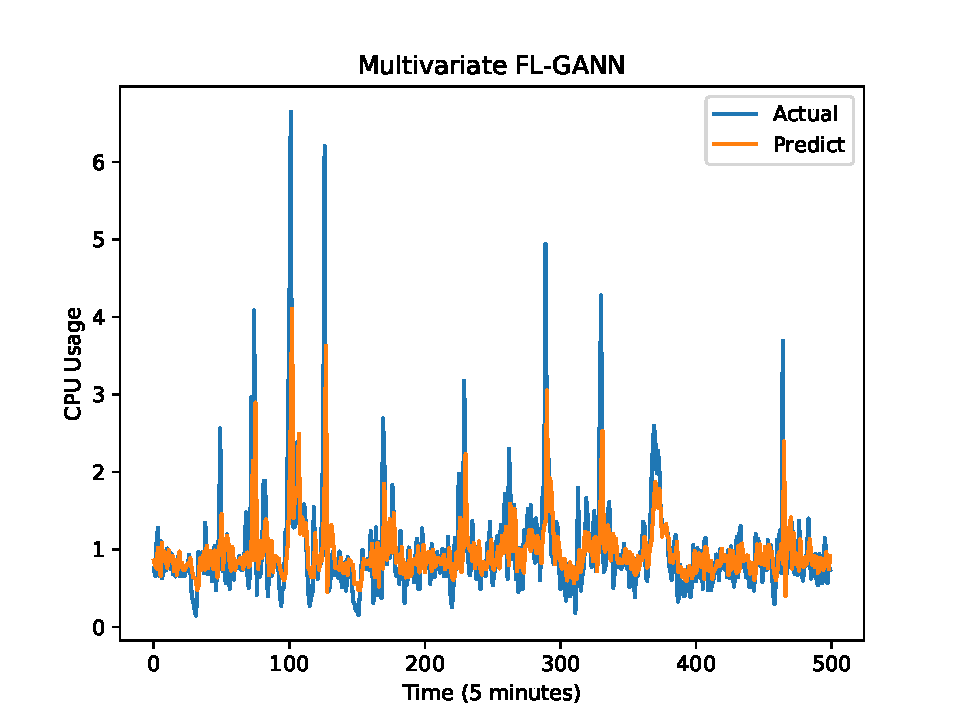
\includegraphics[width=1\textwidth =0cm 0cm 0cm 0cm]{images/pdf/multi_cpu_flgann.pdf}
	\end{minipage}
	\begin{minipage}[t]{4cm}
		\centering
		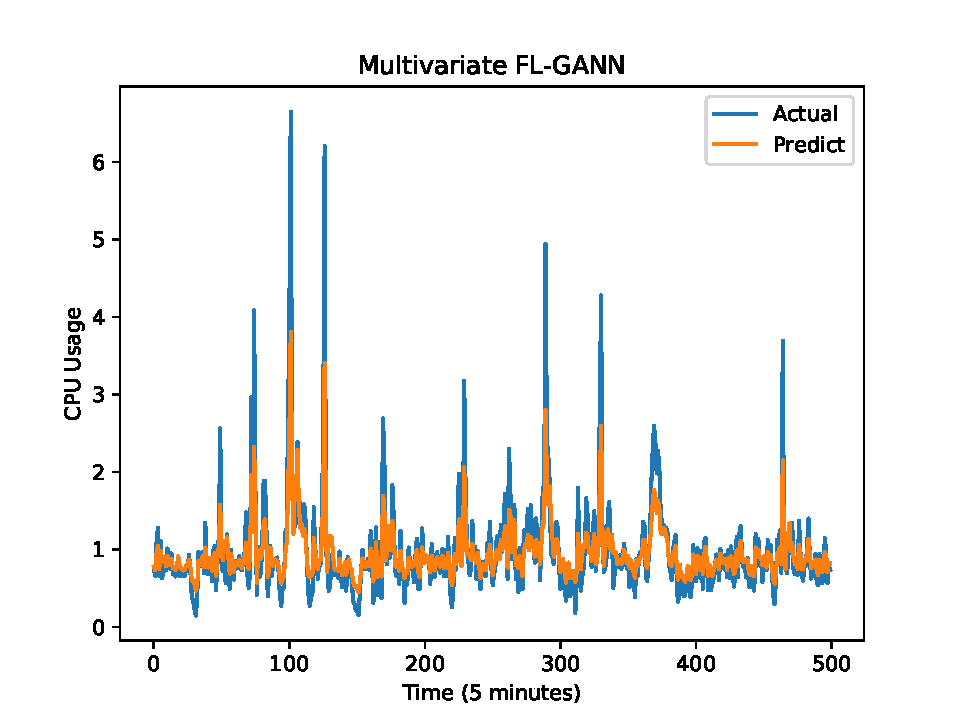
\includegraphics[width=1\textwidth =0cm 0cm 0cm 0cm]{images/pdf/multi_cpu_flbfonn.pdf}
	\end{minipage}
	\begin{minipage}[t]{4cm}
		\centering
		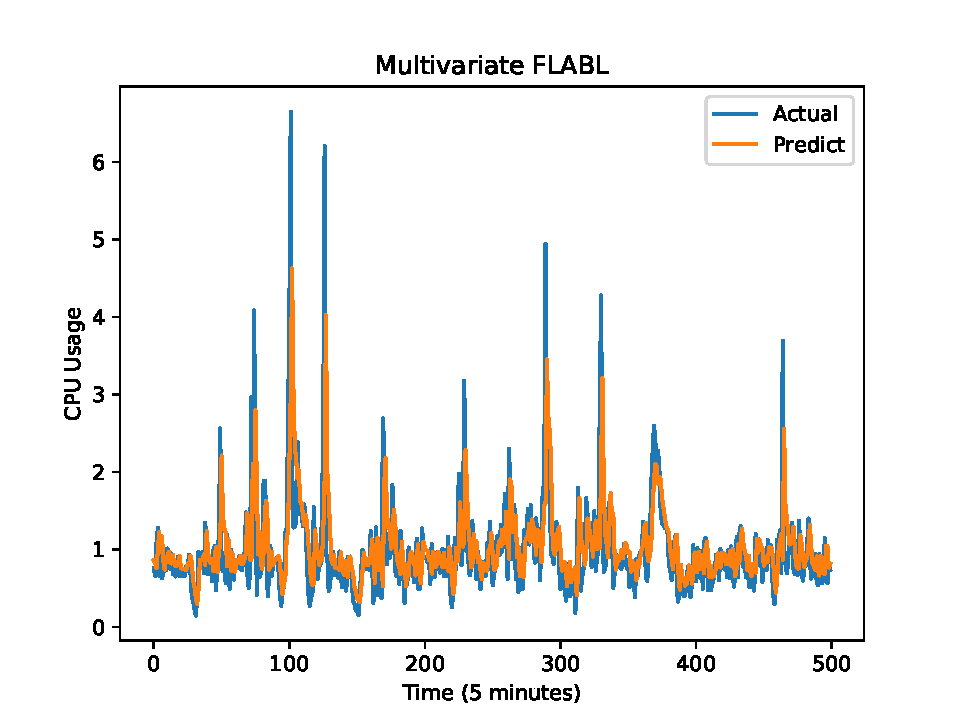
\includegraphics[width=1\textwidth =0cm 0cm 0cm 0cm]{images/pdf/multi_cpu_flabl.pdf}
	\end{minipage}
	\caption{CPU prediction outcomes of FL-GANN (first), FL-BFONN (second) and FLABL (third) with multivariate data, sliding window = 5} 
	\label{tn1_half_multi_CPU}
\end{figure}

\begin{figure}[!h]
	\centering
	\begin{minipage}[t]{4cm}
		\centering
		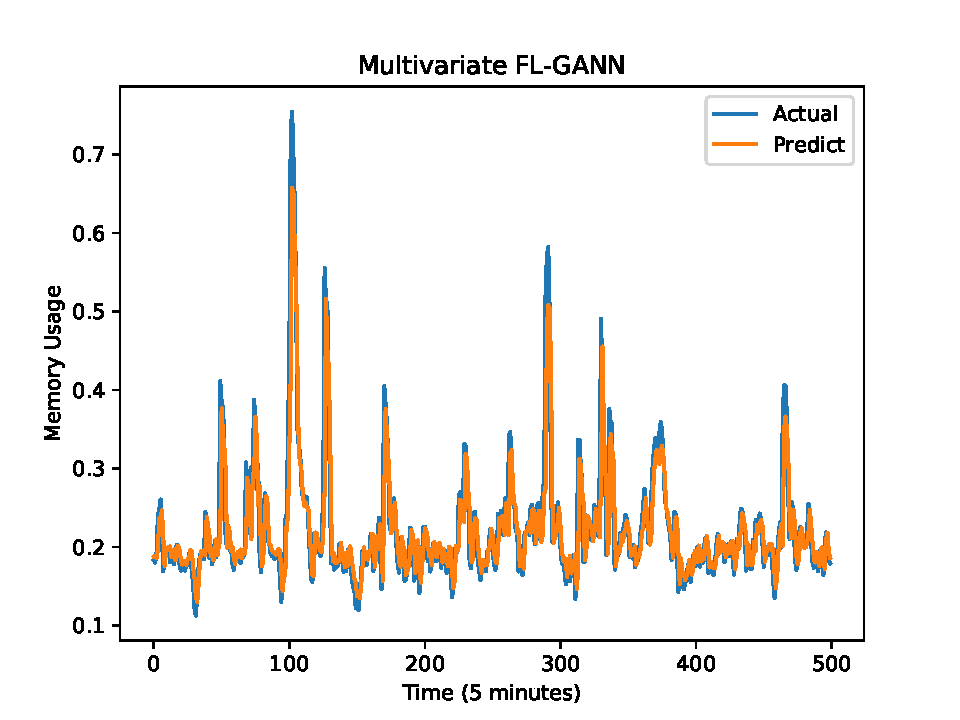
\includegraphics[width=1\textwidth =0cm 0cm 0cm 0cm]{images/pdf/multi_ram_flgann.pdf}
	\end{minipage}
	\begin{minipage}[t]{4cm}
		\centering
		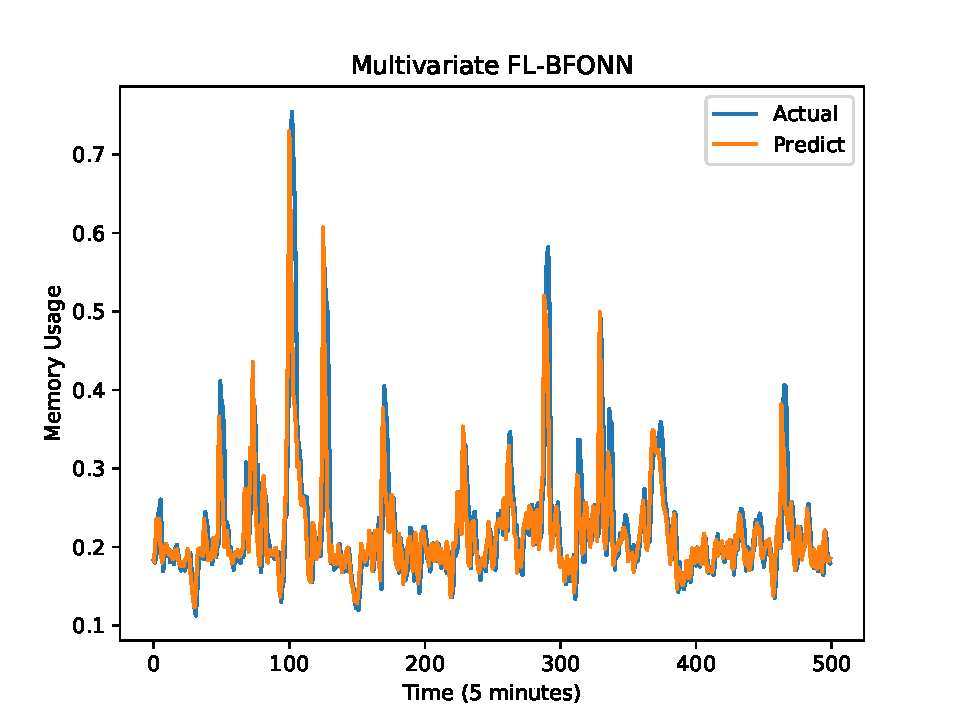
\includegraphics[width=1\textwidth =0cm 0cm 0cm 0cm]{images/pdf/multi_ram_flbfonn.pdf}
	\end{minipage}
	\begin{minipage}[t]{4cm}
		\centering
		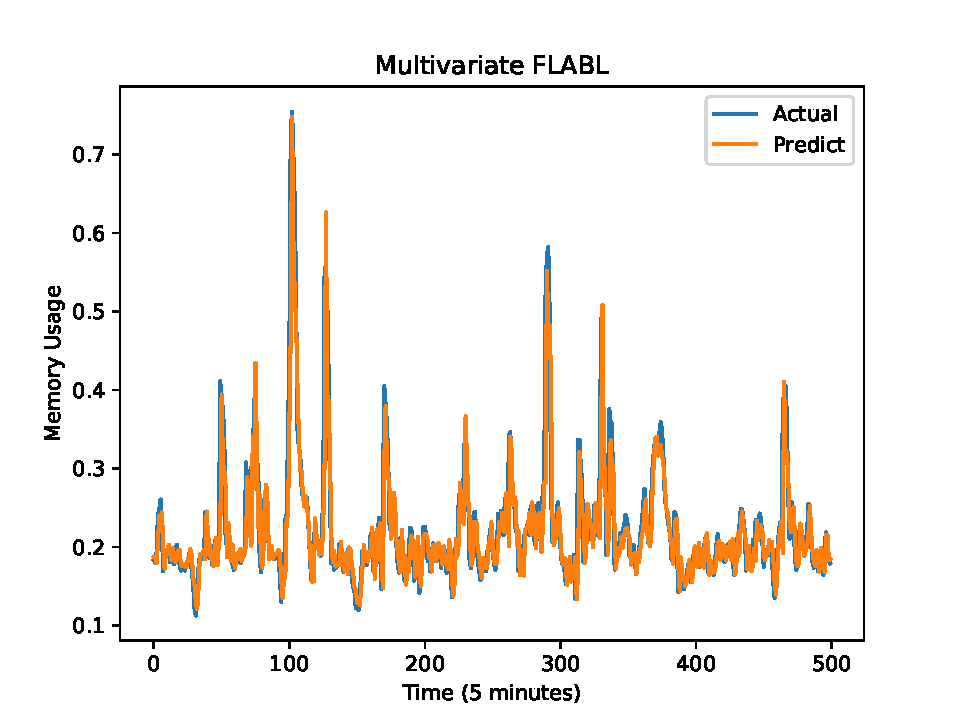
\includegraphics[width=1\textwidth =0cm 0cm 0cm 0cm]{images/pdf/multi_ram_flabl.pdf}
	\end{minipage}
	\caption{Memory prediction outcomes of FL-GANN (first), FL-BFONN (second) and FLABL (third) with multivariate data, sliding window = 5} 
	\label{tn1_half_multi_RAM}
\end{figure}

According to the achieved results, there are some observations that can be made as follows. In almost all cases, RMSE accuracy of FLABL are smaller than ANN, MLNN, traditional FLNN, FL-GANN and FL-BFONN model with different sliding window values as well as input types. Concretely, for univariate data input, FLABL brings the best results as compared with others, also for multivariate data input except $k$ = 4 and 5 in memory prediction case. However, the difference is trivial for the test scenarios (0.0337 (FLABL) compares with 0.0332 (FL-BFONN) with $k$ = 4, and 0.0344 (FLABL) compares with 0.0337(FL-BFONN) with $k$ = 5). This shows the advantage of FLABL in prediction in comparison with other models. Figure~\ref{tn1_half_multi_CPU} and~\ref{tn1_half_multi_RAM} illustrate the prediction outcomes of CPU and memory metrics in accuracy comparison tests among experimental models.

In this test, we compare the speed of those prediction models, which based on 3 factor includes: $t_e$ is average time for 1 epoch (second/epoch), $t_p$ is time to predict test data (second) and $t_s$ is the total time of all system (preprocessing, training and testing - second). Because each model has different epoch configuration, so $t_e$ should be choice instead of the total time of training process.  Our speed comparison are given in Table~\ref{table:time}.

\begin{table}[!h]
\begin{center}
\begin{tabular}{| c | c| C{1.2cm} | C{1.2cm} | C{1.2cm} | C{1.2cm} | C{1.2cm} | C{1.2cm} |}
 \hline
  \multirow{2}{*}{Input Type} & \multirow{2}{*}{Model} & \multicolumn{3}{c|}{CPU} & \multicolumn{3}{c|}{RAM} \\ \cline{3-8}
   & & $t_e$ & $t_p$ & $t_s$ & $t_e$ & $t_p$ & $t_s$  \\ [0.5ex] \hline
 \multirow{5}{*}{ Univariate } & ANN	& 0.0379  & 0.0319  & 198.4  & 0.044 	& 0.0321 	& 220.3  \\ 
 & MLNN	& 0.0583  & 0.0587  & 291.58	& 0.0644 	& 0.0686 	& 322.15  \\   
 & FLNN	& 0.023  & 0.0003  & 114.83 	& 0.0248 	& 0.0003 	& 124.03  \\  
 & FL-GANN	& 0.3154  & 0.0004  & 220.79	& 0.2612 	& 0.0004 	& 182.89  \\ 
 & FL-BFONN	 & 3.473  & 0.0006	& 2778.5 	& 3.289 	& 0.0014  &2521.5 \\ 
 & FLABL	& 0.1095  & 0.0004  & \textbf{71.16}	 & 0.1229	& 0.0007 	& \textbf{122.89}  \\  \hline
  
 \multirow{5}{*}{Multivariate } 	& ANN	 & 0.0406  & 0.0324 	& 202.95	  & 0.0418  & 0.0325 	& 209.15 \\ 
 & MLNN	 & 0.0605  & 0.0598 	& 302.48  & 0.054 & 0.0589	& 270.25 \\ 
 & FLNN	 & 0.0245  & 0.0021 	& 122.53  & 0.0263 & 0.0004	& 131.45 \\ 
 & FL-GANN	 & 0.3944  & 0.0004 	& 276.15   & 0.4176  &  0.0004 	& 292.35 \\ 
 & FL-BFONN	 & 3.166  & 0.0007 	& 2532.6   & 3.177  &  0.0034 	& 2541.5 \\ 
 & FLABL	 & 0.1708  & 0.0008 	 &170.82   & 0.1419 & 0.0009	  & 141.91   \\ \hline 
\end{tabular}
\end{center}
\caption{System run time (second) comparison between FLABL and other models with sliding window = 5}
\label{table:time}
\end{table}

\subsection{Auto-scaling strategy}
\label{decision_results}
In this test, we evaluate auto-scaling decisions made based on prediction results and SLA violation assessments as presented in Subsection~\ref{decision_module}. Figure~\ref{fig_scaling_1013} shows the number of VMs calculated using the formula~\ref{eq_vm_allocated}. An observation can be made from the obtained outcomes as follows. With $s <$  1.3, there are still some under-provision VMs as compared with resource requirements. For $s$ $\geq$ 1.3, VMs are allocated sufficiently for the demand usages. It's also shown in below test when we consider the lack and over-provision of resources. 

In order to assess the lack or over-provision of resources, we use SLAVTP and ADI measurements. 
%The evaluation results are presented in Table~\ref{table:scaling_vio} and~\ref{table:scaling_adi}.
%For the lack of resources issue (the resources amount allocated to applications is smaller than actual requirements), based on SLAVTP evaluation formulation, 
Concretely, table~\ref{table:scaling_vio} shows SLAVTP estimations of various models in VM allocation process with window size $p$ = 3. In general, our proposed model gains smaller SLAVTP values than other models when the scaling coefficient is changed. For example, when $s$ = 2.0, FLABL univariate model has only 0.18$\%$ violation, while the multivariate model violates 0.12$\%$. Especially, when $s$ = 2.5 both of univariate and multivariate model reaches 0$\%$ violation. Of course, in these cases, the number of VMS provisioned is quite large.

\begin{figure}[!h]
	\centering
	\begin{minipage}[t]{6cm}
		\centering
		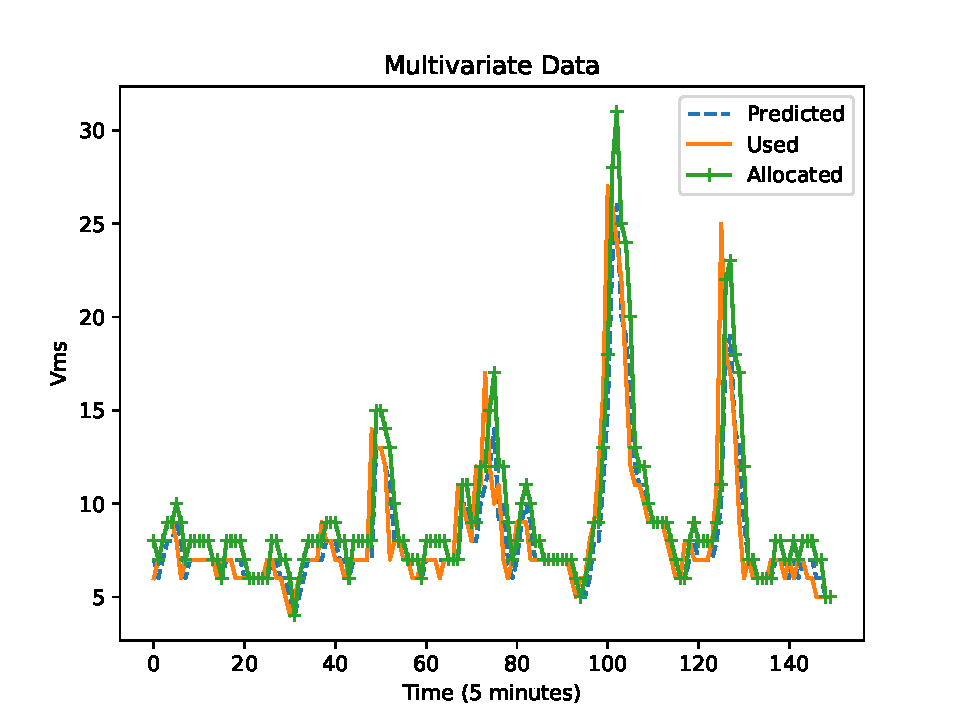
\includegraphics[width=1\textwidth =0cm 0cm 0cm 0cm]{images/pdf/scaling/fl_bfonn_vms-s_10-L_5.pdf}
	\end{minipage}
	\begin{minipage}[t]{6cm}
		\centering
		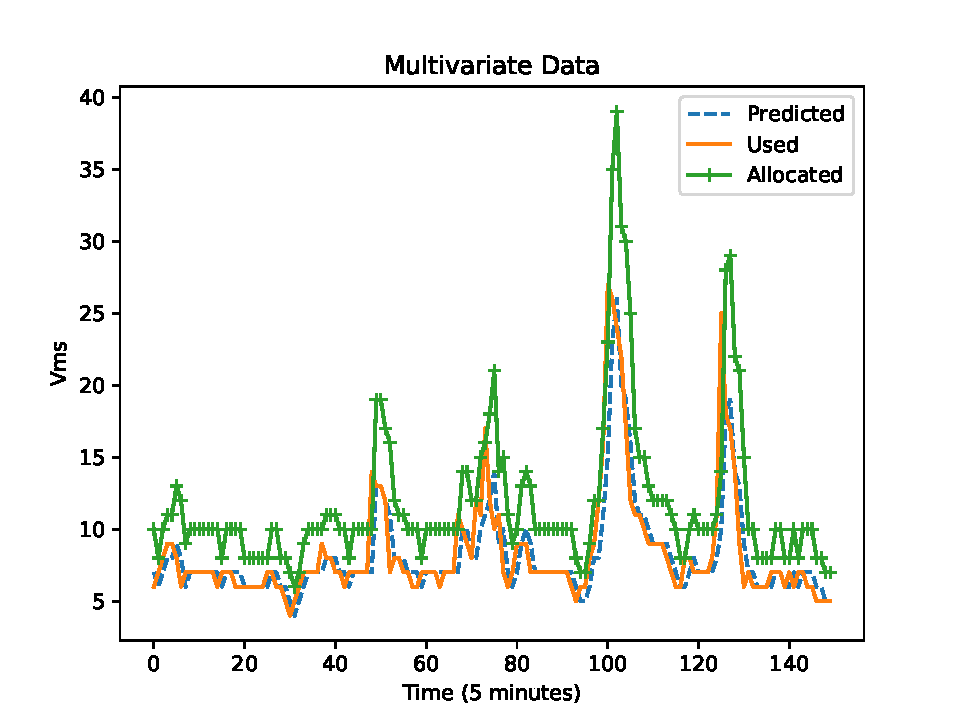
\includegraphics[width=1\textwidth =0cm 0cm 0cm 0cm]{images/pdf/scaling/fl_bfonn_vms-s_13-L_5.pdf}
	\end{minipage}
	\caption{The number of predicted, allocated, used VMs with sliding window = 3, adaptation length $L$ = 5, and scaling coefficient $s$ = 1 (left), $s$ = 1.3(right)} 
	\label{fig_scaling_1013}
\end{figure}

\begin{table}[!h]
	\begin{center}
		\begin{tabular}{| c | c| C{1.1cm} | C{1.1cm} | C{1.1cm} | C{1.1cm} | C{1.1cm} | C{1.1cm} | C{1.1cm} |}
			\hline
			\multirow{2}{*}{Input Type} & \multirow{2}{*}{Model} & \multicolumn{7}{c|}{scaling coefficient} \\ \cline{3-9}
			& & s = 1.0 & s = 1.3 & s = 1.5 & s = 1.7 & s = 2.0 & s = 2.2 & s = 2.5  \\ [0.5ex] \hline
			\multirow{5}{*}{ Univariate } & ANN	& 10.3  &1.87  &1.02  &0.54  &0.18  &0.12  &0.06  \\  
			& MLNN	 &10.24	&1.81	&0.96	&0.6 	&0.18	&0.12	&0.06 \\ 
			& FLNN  &9.28  &1.81  &0.96  &0.54  &0.24  &0.24  &0.12  \\
			&FL-GANN &11.33 &1.69  &0.9  &0.48  &0.24  &0.18  &0.06  \\
			& FL-BFONN & 11.81  &1.75 &0.84  &0.54  &0.24  &0.06  &0  \\
			&FLABL &10.3  &1.93  &1.02 &0.54  &\textbf{0.18}  &\textbf{0.06}  &\textbf{0} \\ \hline
			
			\multirow{5}{*}{Multivariate} & ANN &15.96 &7.59  &5.42  &4.28  &3.13  &2.53  &1.99   \\ 
			& MLNN &10.42  &1.69  &0.9  &0.6  &0.18  &0.06  &0.06\\
			& FLNN &11.08  &1.75  &0.84  &0.54  &0.12 &0.06  &0 \\
			& FL-GANN &10.3  &1.69  &1.27  &0.48  &0.24  &0.12  &0.06 \\
			& FL-BFONN	 &9.7	&1.81	&0.84	&0.6 	&0.18	&0.12	&0.06 \\
			& FLABL &\textbf{9.76} &\textbf{1.69}  &0.9  &0.54  &\textbf{0.12}  &\textbf{0.06}  &\textbf{0} \\ \hline
		\end{tabular}
	\end{center}
	\caption{Violation percentage in comparison among various models with adaptation length = 5, and sliding window = 3}
	\label{table:scaling_vio}
\end{table}

\begin{table}[!h]
	\begin{center}
		\begin{tabular}{| c | c| C{1.1cm} | C{1.1cm} | C{1.1cm} | C{1.1cm} | C{1.1cm} | C{1.1cm} | C{1.1cm} |}
			\hline
			\multirow{2}{*}{Input Type} & \multirow{2}{*}{Model} & \multicolumn{7}{c|}{scaling coefficient} \\ \cline{3-9}
			& & s = 1.0 & s = 1.3 & s = 1.5 & s = 1.7 & s = 2.0 & s = 2.2 & s = 2.5  \\ [0.5ex] \hline
			\multirow{5}{*}{ Univariate } & ANN	&154.01  &15.41  &37.88  &112.63  &227.11 &293.53  &372.4 \\   
 			& MLNN  &176.59  &3.81  &4.87  &78.94  &205.75  &270.58  &353.31 \\
			&FLNN & 184.6  &4.41  &11.29  &82.46 &207.8 &277.2 &357.88  \\
			&FL-GANN &176.67  &3.86  &15.9  &89.18  &214.8  &283.6 &363.81 \\
			&FL-BFONN & 179.62 &5.21  &4.42  &77.31  &202.46  &267.21  &350.03 \\
			&FLABL &189.27  &\textbf{3.7}  &5.54  &74.73  &\textbf{199.9}  &\textbf{267}  &\textbf{349.5} \\ \hline
			
			\multirow{5}{*}{Multivariate} &ANN &342.11  &320.86  &356.43  &394.72 & 456.56  &491.43  &539.16  \\ 
			&MLNN &203.73  &10.03  &7.84  &67.19  &192.52   &254.28  &337.38 \\
			&FLNN &183.2  &8.63  &14.53  &83.34  &203.7  &271.43  &352.82 \\
			&FL-GANN &195.78  &9.79  &10.24  &74.45  &192.43 &259.98   &341.88 \\
			&FL-BFONN &219.81 &40.24 &36.47 &93.23  &197.92  &260.28  &340.58    \\
			& FLABL	 &192.27	 &\textbf{8.22}	&\textbf{5.5}	 &72.16 	&\textbf{183.9}	 &259.61	&342.76  \\ \hline
		\end{tabular}
	\end{center}
	\caption{ADI in comparison among various models with adaptation length = 5, and sliding window = 3}
	\label{table:scaling_adi}
\end{table}

Based on the ADI measurement, table~\ref{table:scaling_adi} shows the ADI evaluation of different predictive models, with the desired utilization [60$\%$, 80$\%$] and window size $p$ = 3. It is easy to observe that ADI of FLABL for both univariate and multivariate data types is smaller than others. Specifically, in the test, optimal ADI is at 3.7 when $s$ = 1.3. The results demonstrate significant effect of our prediction as well as decision solutions. As mentioned above, when $s$ is increased, SLA violation decreases but resource over-provision phenomenon occurs.



\section{Conclusion and future work}
\label{conclusion}

In this paper, we presented our designs for a novel cloud proactive auto-scaler with complete modules from prediction to decision making. Thus, functional-link neural network is used for the forecast phase. To overcome back-propagation drawback, we integrate adaptive bacterial foraging life-cycle and social learning optimization with the artificial neural network. This improvement brings better accuracy for our proposed model. The auto-scaler designed in this paper also enables the capability of analyzing multiple monitoring metrics at the same time. This mechanism supports our system to be able to discover the implicit relationships among metrics types and thus help make scaling decisions more precisely. For the decision module, we proposed an efficient way to calculate the number of VMs that are provided for cloud-based applications using SLA violation measurement. We tested the auto-scaler with a real dataset generated by Google cluster. The obtained outcomes show that our system can work efficiently as compared with other methods and it can be applied to practice in clouds. For the future, we would like to implement the auto-scaler in private cloud middleware like Openstack or OpenNebula. Based on the infrastructures, we will test the proposal with applications under real conditions.


\section*{Acknowledgments} This research is supported by 
Vietnamese MOETs project ``Research on developing software framework to integrate IoT gateways for fog computing deployed on multi-cloud environment'' No. B2017-BKA-32,
Slovak APVV-17-0619 ``Urgent Computing for Exascale Data'', and
EU H2020-777536 EOSC-hub ``Integrating and managing services for the European Open Science Cloud''.


% ---- Bibliography ----
%
% BibTeX users should specify bibliography style 'splncs04'.
% References will then be sorted and formatted in the correct style.
%
\bibliographystyle{splncs04}
\bibliography{references}


\end{document}
